\documentclass{standalone}
\usepackage{tikz,calc}
\usetikzlibrary{bending,positioning}


\begin{document}
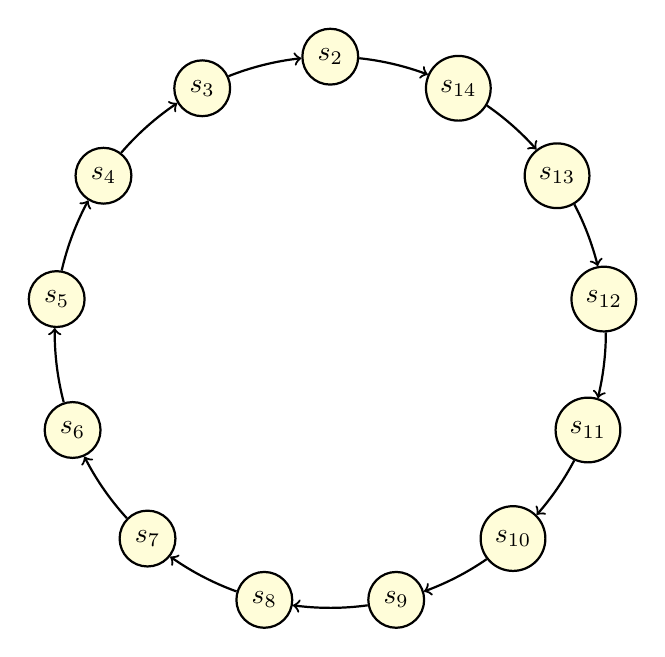
\begin{tikzpicture}[
  ->,
  thick,
   main node/.style={draw,circle,fill=yellow!15},
]
  \newcommand*{\MainNum}{13}
  \newcommand*{\MainRadius}{3.5cm}
  \newcommand*{\MainStartAngle}{90}

  % Print main nodes, node names: p1, p2, ...
  \path
    (0, 0) coordinate (M)
    \foreach \t [count=\i] in {2,...,14} {
      +({\i-1)*360/\MainNum + \MainStartAngle}:\MainRadius)
      node[main node, align=center] (s_\i) {$s_{\t}$}
    }
  ;



  % Calculate the angle between the equal sides of the triangle
  % with side length \MainRadius, \MainRadius and radius of circle node
  % Result is stored in \p1-angle, \p2-angle, ...
  \foreach \i in {1, ..., \MainNum} {
    \pgfextracty{\dimen0 }{\pgfpointanchor{s_\i}{north}}
    \pgfextracty{\dimen2 }{\pgfpointanchor{s_\i}{center}}
    \dimen0=\dimexpr\dimen2 - \dimen0\relax
    \ifdim\dimen0<0pt \dimen0 = -\dimen0 \fi
    \pgfmathparse{2*asin(\the\dimen0/\MainRadius/2)}
    \global\expandafter\let\csname p\i-angle\endcsname\pgfmathresult
  }

  % Draw the arrow arcs
  \foreach \i [evaluate=\i as \nexti using {int(mod(\i, \MainNum)+1}]
  in {1, ..., \MainNum} {
    \pgfmathsetmacro\StartAngle{
      (\i-1)*360/\MainNum + \MainStartAngle
      + \csname p\i-angle\endcsname
    }
    \pgfmathsetmacro\EndAngle{
      (\nexti-1)*360/\MainNum + \MainStartAngle
      - \csname p\nexti-angle\endcsname
    }
    \ifdim\EndAngle pt < \StartAngle pt
      \pgfmathsetmacro\EndAngle{\EndAngle + 360}
    \fi
    \draw[<-]
      (M) ++(\StartAngle:\MainRadius)
      arc[start angle=\StartAngle, end angle=\EndAngle, radius=\MainRadius]
    ;
  }

\end{tikzpicture}
\end{document}


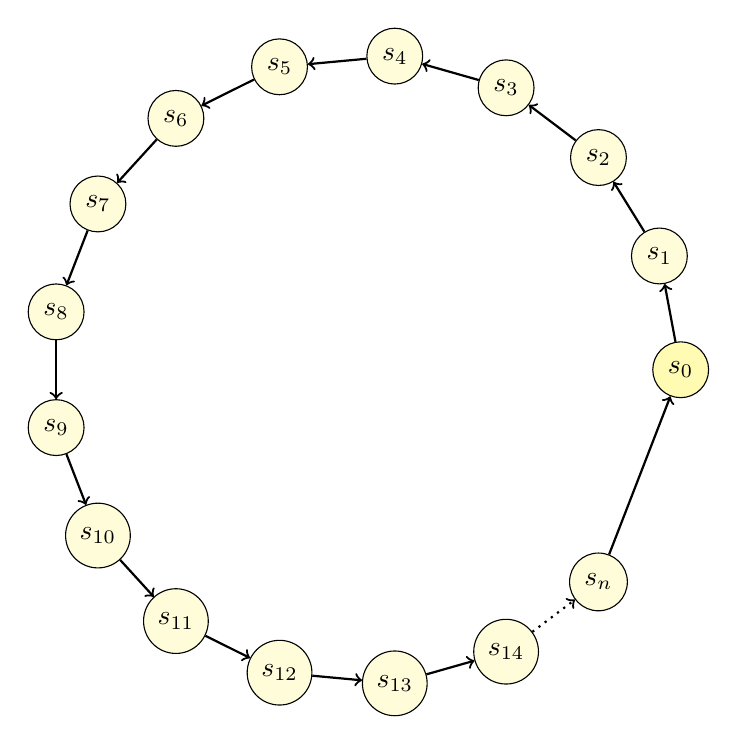
\begin{tikzpicture}
\tikzstyle{s}=[draw,circle,fill=yellow!15]
   \draw (1*360/17: 4cm) node (s1) [s] {$s_{1}$};
   \draw (2*360/17: 4cm) node (s2) [s] {$s_{2}$};
   \draw (3*360/17: 4cm) node (s3) [s] {$s_{3}$};
   \draw (4*360/17: 4cm) node (s4) [s] {$s_{4}$};
   \draw (5*360/17: 4cm) node (s5) [s] {$s_{5}$};
   \draw (6*360/17: 4cm) node (s6) [s] {$s_{6}$};
   \draw (7*360/17: 4cm) node (s7) [s] {$s_{7}$};
   \draw (8*360/17: 4cm) node (s8) [s] {$s_{8}$};
   \draw (9*360/17: 4cm) node (s9) [s] {$s_{9}$};
   \draw (10*360/17: 4cm) node (s10) [s] {$s_{10}$};
   \draw (11*360/17: 4cm) node (s11) [s] {$s_{11}$};
   \draw (12*360/17: 4cm) node (s12) [s] {$s_{12}$};
   \draw (13*360/17: 4cm) node (s13) [s] {$s_{13}$};
   \draw (14*360/17: 4cm) node (s14) [s] {$s_{14}$};

   \draw (360: 4cm) node (s0) [s,fill=yellow!30] {$s_{0}$};
   \draw (15*360/17: 4cm) node (sn) [s] {$s_{n}$};
   \path [draw,thick,->] (sn) -- (s0) ;
   \path [draw,thick,->] (s0) -- (s1) ;
   \path [draw,thick,->] (s1) -- (s2) ;
   \path [draw,thick,->] (s2) -- (s3) ;
   \path [draw,thick,->] (s3) -- (s4) ;
   \path [draw,thick,->] (s4) -- (s5) ;
   \path [draw,thick,->] (s5) -- (s6) ;
   \path [draw,thick,->] (s6) -- (s7) ;
   \path [draw,thick,->] (s7) -- (s8) ;
   \path [draw,thick,->] (s8) -- (s9) ;
   \path [draw,thick,->] (s9) -- (s10) ;
   \path [draw,thick,->] (s10) -- (s11) ;
   \path [draw,thick,->] (s11) -- (s12) ;
   \path [draw,thick,->] (s12) -- (s13) ;
   \path [draw,thick,->] (s13) -- (s14) ;

   \path [draw,thick,->,dotted] (s14) -- (sn) ;
\end{tikzpicture}
\end{document}
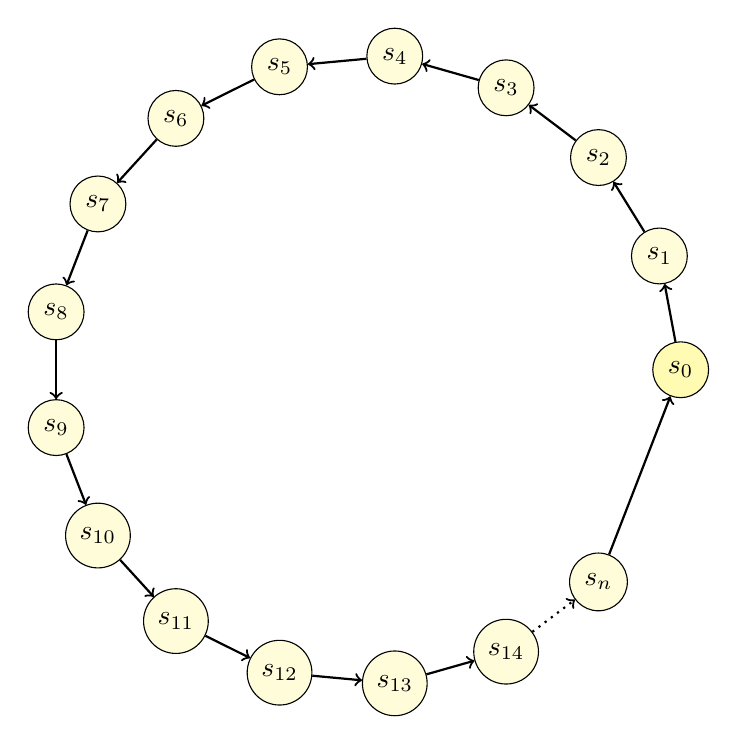
\begin{tikzpicture}
\tikzstyle{s}=[draw,circle,fill=yellow!15]
   \draw (1*360/17: 4cm) node (s1) [s] {$s_{1}$};
   \draw (2*360/17: 4cm) node (s2) [s] {$s_{2}$};
   \draw (3*360/17: 4cm) node (s3) [s] {$s_{3}$};
   \draw (4*360/17: 4cm) node (s4) [s] {$s_{4}$};
   \draw (5*360/17: 4cm) node (s5) [s] {$s_{5}$};
   \draw (6*360/17: 4cm) node (s6) [s] {$s_{6}$};
   \draw (7*360/17: 4cm) node (s7) [s] {$s_{7}$};
   \draw (8*360/17: 4cm) node (s8) [s] {$s_{8}$};
   \draw (9*360/17: 4cm) node (s9) [s] {$s_{9}$};
   \draw (10*360/17: 4cm) node (s10) [s] {$s_{10}$};
   \draw (11*360/17: 4cm) node (s11) [s] {$s_{11}$};
   \draw (12*360/17: 4cm) node (s12) [s] {$s_{12}$};
   \draw (13*360/17: 4cm) node (s13) [s] {$s_{13}$};
   \draw (14*360/17: 4cm) node (s14) [s] {$s_{14}$};

   \draw (360: 4cm) node (s0) [s,fill=yellow!30] {$s_{0}$};
   \draw (15*360/17: 4cm) node (sn) [s] {$s_{n}$};
   \path [draw,thick,->] (sn) -- (s0) ;
   \path [draw,thick,->] (s0) -- (s1) ;
   \path [draw,thick,->] (s1) -- (s2) ;
   \path [draw,thick,->] (s2) -- (s3) ;
   \path [draw,thick,->] (s3) -- (s4) ;
   \path [draw,thick,->] (s4) -- (s5) ;
   \path [draw,thick,->] (s5) -- (s6) ;
   \path [draw,thick,->] (s6) -- (s7) ;
   \path [draw,thick,->] (s7) -- (s8) ;
   \path [draw,thick,->] (s8) -- (s9) ;
   \path [draw,thick,->] (s9) -- (s10) ;
   \path [draw,thick,->] (s10) -- (s11) ;
   \path [draw,thick,->] (s11) -- (s12) ;
   \path [draw,thick,->] (s12) -- (s13) ;
   \path [draw,thick,->] (s13) -- (s14) ;

   \path [draw,thick,->,dotted] (s14) -- (sn) ;
\end{tikzpicture}
